The collaborative side of the algorithm starts by receiving a single user, and afterwards gets all different users and puts them into a collection. The algorithm indexes the user, creating a dictionary, which contains pairs of a user from the collection, together with a coefficient based on the linear similarity between them and the main user. This coefficient is based on the Pearson correlation coefficient which has previously been described in Section \ref{CollaborativeDes}.

\subsubsection{Pearson}

The two sets that is needed for each Pearson calculation, is the ratings of media items, which both the main and secondary user have in common in their medialist. The Pearson calculation will then return a coefficient based on these two collections of ratings, indicating how similar they are in their ratings, and general rating habits. Following this, users with negative or no correlation will be removed, and the remaining is sorted by their given coefficient, going from highest to lowest. See Figure \ref{PearsonCalc} for the Pearson calculation.

\begin{table}[htb]
\centering
\begin{tabular}{|l|l|l|l|l|} \hline
	\textbf{$x$} & \textbf{$y$} & \textbf{$xy$}
	& \textbf{$x^2$} & \textbf{$y^2$} \\ \hline
	2 & 3 & 6 & 4 & 9 \\ \hline
	4 & 5 & 20 & 16 & 25 \\ \hline
	6 & 5 & 30 & 36 & 25 \\ \hline
	8 & 7 & 56 & 64 & 49 \\ \hline\hline
	20 & 20 & 112 & 120 & 108 \\ \hline
\end{tabular}
\caption{Pearson Example}
\label{PearsonEx}
\end{table} 

In Table \ref{PearsonEx} is two sets of ratings, $x$ and $y$, which is then put together to create 5 sums, that also can be seen above. These sums is then used as the parameters for the Pearson calculation, together with the number of pairs, which is 4. In this example Pearson returns $0,949$, a very good coefficient. See Listing \ref{CompareUserPairTwo} for the part of the algorithm that finds these coefficients.

\begin{lstlisting}[caption={The CompareUserPair method},label={CompareUserPairTwo}]
private double CompareUserPair(User mainUser, User user)
{
	List<int> mainRating = new List<int>();
	List<int> userRating = new List<int>();
	int x = 0, y = 0, xy = 0, x2 = 0, y2 = 0;

	foreach (Media media in user.MediaList.Keys)
	{
		if (mainUser.MediaList.ContainsKey(media))
		{
			mainRating.Add(mainUser.MediaList[media]);
			userRating.Add(user.MediaList[media]);
		}
	}

	if (mainRating.Count() < 3)
	{
		return 0;
	}

	for (int i = 0; i < mainRating.Count; i++)
	{
		x += mainRating[i];
		y += userRating[i];
		xy += mainRating[i] * userRating[i];
		x2 += (int)Math.Pow(mainRating[i], 2);
		y2 += (int)Math.Pow(userRating[i], 2);
	}

	return Pearson(x, y, xy, x2, y2, mainRating.Count());
}
\end{lstlisting}

The initial loop runs through the main users medialist, and if the secondary user have the same media in their medialist, their ratings will be added to two lists. If this loop could not find more than two media matches, the method will return 0. If you only have two sets of ratings, Pearson will always return either $-1$, $0$, or $1$, which is not a precise coefficient for how similar they, and may result in wrong recommendations. As seen in Section \ref{CollaborativeDes}, Pearson tries to make a line of best fit between two sets of data, and if there is only two points in their graph representation, the line will always be a perfect fit. 


The parameters for the Pearson's calculation is then determined through another loop, if there was enough rating pairs to work with. The result of Pearson will then be returned. Another problem with Pearson happens when all ratings extracted from one user is identical. For example, if every element in $y$ from Table \ref{PearsonEx} is 5. If this happens, Pearson cannot create a proper coefficient, and will return NaN, not a number. These users who is assigned NaN is later discarded. This may mean users with good coefficients can end up being ignored.

\subsubsection{Recommendation Extraction}

After every user have been assigned a coefficient the next part of the algorithm begins. This part extracts media from the rated users medialists, and returns these media as recommendations. See Figure \ref{CollaEx} for an example of this process.

\begin{figure}[H]
\centering
\begin{subfigure}{.5\textwidth}
  \centering
  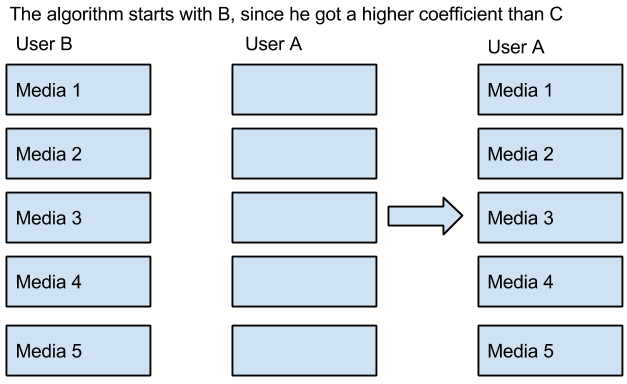
\includegraphics[width=.9\linewidth]{Images/CollaborativeRecExample1.png}
  \caption{}
  \label{fig:collarec1}
\end{subfigure}%
\begin{subfigure}{.5\textwidth}
  \centering
  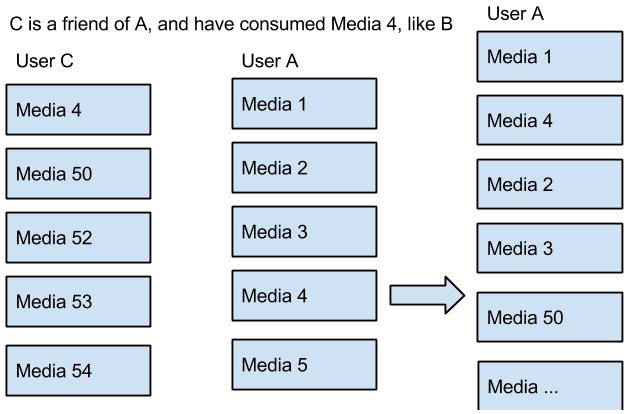
\includegraphics[width=.9\linewidth]{Images/CollaborativeRecExample2.png}
  \caption{}
  \label{fig:collarec2}
\end{subfigure}
\caption{Example showing the collaborative selection process}
\label{CollaEx}
\end{figure}

In Figure \ref{CollaEx}, user A is the user which the algorithm is trying to generate recommendations for. User B and C have both been assigned a coefficient, where B’s coefficient is higher. The algorithm will begin adding media from B’s medialist he have rated higher than a certain threshold to a collection. This collection will then be returned as the generated recommendations, as seen on Figure \ref{fig:collarec1}.

Once the algorithm begins looking through user C, there have already been added several media to the recommendation list as seen on \ref{fig:collarec2}. Users with higher coefficients will always take precedence, and so does their media in the recommendation list. This may change in two scenarios: If the same media appears in an other users medialist, or if a user is friends with the main user. In Figure \ref{fig:collarec2}, media 4 appears again, which boosts it up the recommendation list by one. Because C is friends with A, media 4 is boosted yet again by one. All other media is also boosted by one because of this friendship relation, effectively giving media from user C an advantage. Through this extraction the returned media follows three priorities: first by highest rated user, second by if the same media have already been added, and third by whether or not the user is a friend.